\section{Emitter EPS}
\label{emitter_EPS}

\chapter{Emitter EPS}
\label{emitter_EPS}

The electrical power subsystem for the emitter is almost the same as that for the receiver. There are, however, some differences which will be explained here. The first difference is that the power requirement is much higher. This leads to a larger solar panel area and correspondingly more batteries. The receiver had one battery consisting of two modules, which in turn had seven lithium-ion cells each. The emitter has three of these batteries. 
The other subparts remain the same for the emitter satellite.
As with the receiver satellite, the assumed cosine loss was checked with the STK program. During the preliminary design, the 117W power requirement of the emitter led to a total solar panel area of 1.4 square meters. The STK program calculated that the average power generation of this area was 147W. Again, the assumed cosine loss was proven to be a correct assumption. Figure \ref{fig:powersim} shows the simulated power generation for one typical day. As can be seen, there are 15 orbits every day with eclipse periods in betweeen where there is no power generations.

\begin{figure}[H!]
\centering
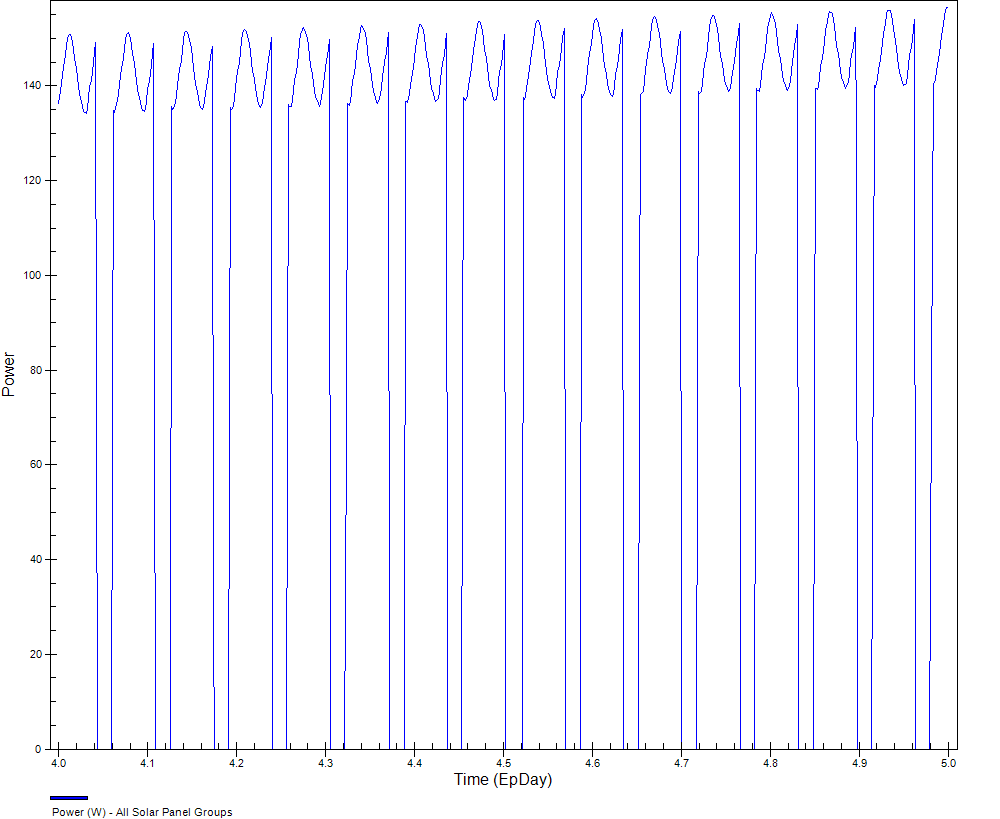
\includegraphics{img/powerSim.png}
\caption{Simulated power generation of emitter satellite solar panels}
\label{fig:powersim}
\end{figure}


The next table shows the dimensions, weight and power usage of each part of the emitter satellite's electrical power system.


\begin{table}[H!]
\centering
\begin{tabular}{cccccc}
\toprule
Part & \multicolumn{3}{c}{Dimensions [mm]} & Weight [g] & Power usage [W]\\ 
\midrule
 & Length & Width & Height & & \\ 
 Drivers (2) & 30 & 6 & 60 & 21.4 & 1 \\ 
 SMA Deployment (2) & 120 & 50 & 10 & 120 & 4* \\ 
 Battery (3) & 168 & 102 & 10 & 1000 & 0 \\ 
 Convertor & 95 & 60 & 17 & 80 & 1.5 \\ 
 Shunt regulator (2) & 2.8 & 2.6 & 1.05 & 0.1 & 0.5 \\ 
 Thermal knife (2) & 60 & 50 & 38 & 280 & 15**  \\
 Wiring & - & - & - & 1219 & 1.7 \\ 
 Solar panels (2) & 1200 & 600 & 7.5 & 600 & 0 \\
 \midrule
 TOTAL & - & - & - & 2593.5 & 3.28***  \\ 
\bottomrule
 \multicolumn{6}{l}{* for 4 minutes} \\
 \multicolumn{6}{l}{** for 60 seconds} \\
 \multicolumn{6}{l}{*** continuous power usage only} \\
\end{tabular}
\caption{EPS subpart details for receiver satellites}
\label{tab:EPS_details}
\end{table}